\section{Softwaretests}\label{text:Entwicklung-der-GFA:Softwaretests}

Die Softwaretests sind ein wichtiger Bestandteil der Softwareentwicklung. Sie dienen dazu, die Funktionalität der Software zu überprüfen und Fehler zu finden. In diesem Abschnitt werden die Softwaretests für die Gleisfreimeldeanlage beschrieben.\newline
Die Tests für die Gleisfreimeldeanlage sind Software-seitig in zwei Kategorien unterteilt:
\begin{itemize}
    \item Tests für Geraden
    \item Tests für Weichen
\end{itemize}
Die Test-Skripte wurden nach und nach entwickelt und immer wieder ausgeführt. Somit wurden zunächst die Methoden zur Initialisierung der einzelnen Komponenten getestet und später die Methoden zur Überprüfung der Funktionalität der Gleisfreimeldeanlage.

\subsection{Tests für Geraden}\label{text:Entwicklung-der-GFA:Softwaretests:Tests-für-Geraden}

Das Testprogramm startet mit der Initialisierung der einzelnen Komponenten. Da das Skript zu lange ist um es hier komplett darzustellen, wird nur ein Ausschnitt dessen gezeigt. Für das Verständnis ist es wichtig die folgenden Definitionen zu kennen:
\begin{itemize}
    \item p1, p2, p3, p4 sind Kontaktpunkte
    \item d1 ist ein gerichteter Achszähler, der die Kontaktpunkte p1 und p2 verwendet
    \item d2 ist ein gerichteter Achszähler, der die Kontaktpunkte p3 und p4 verwendet
    \item c ist ein Counter/ Streckenabschnitt
    \item v ist die Gleisfreimeldeanlage
\end{itemize}

Das Testprogramm testet die folgenden Fälle:\footnote{Die Fälle, die mit einem * markiert sind, erwarten einen Fehler}
\begin{itemize}
    \item Ein Zug fährt normal über die Gerade 
    \item Ein Zug fährt rückwärts über die Gerade
    \item Ein Zug ändert unangekündigt die Richtung im Streckenabschnitt*
    \item Ein Zug fährt aus einem Streckenabschnitt, ohne in diesen eingefahren zu sein*
    \item Ein Zug mit mehreren Achsen fährt über die Gerade
    \item Ein Zug fährt über die Gerade, wendet und fährt wieder zurück
\end{itemize}

Beim Testen der Geraden wird die Methode \texttt{rail\_vacancy\_assert} verwendet, um die Funktionalität der Gleisfreimeldeanlage zu überprüfen. Diese Methode erwartet als Parameter die Gleisfreimeldeanlage, ein Array von Kontaktpunkten und die Anzahl der Kontaktpunkte. Die Methode triggert die Kontaktpunkte in der Reihenfolge, in der sie im Array übergeben wurden und überprüft, dass kein Fehler auftritt.\newline 
Die Methode \texttt{rail\_vacancy\_assert\_error} erwartet zusätzlich den Fehlercode, der erwartet wird. Diese Methode wird verwendet, um Fehler zu testen, die auftreten, wenn ein Zug unangekündigt die Richtung ändert oder aus einem Streckenabschnitt fährt, ohne in diesen eingefahren zu sein.\newline 
Die Methode \texttt{rail\_vacancy\_assert\_with\_change} erhält zwei Arrays von Kontaktpunkten. In dieser Methode werden zunächst die Kontaktpunkte im ersten Array getriggert, dann wird die Funktion zum Ändern der Richtung aufgerufen und anschließend die Kontaktpunkte im zweiten Array getriggert. Diese Methode wird verwendet, um zu testen, ob die Gleisfreimeldeanlage korrekt reagiert, wenn ein Zug die Richtung ändert. Der Ausschnitt des Testprogramms ist in \autoref{lst:Testprogramm} dargestellt.

\begin{lstlisting}[caption={Ausschnitt des Testprogramms für Geraden},label={lst:Testprogramm},language=C]
  printf("Test normal route\n");
  rail_vacancy_assert(v, (rail_contact_point_t *[]){p1, p2, p3, p4}, 4);
  rail_contact_counter_reset(c);

  printf("Test reverse route\n");
  rail_vacancy_assert(v, (rail_contact_point_t *[]){p4, p3, p2, p1}, 4);
  rail_contact_counter_reset(c);

  printf("Test change in direction (results in error)\n");
  rail_vacancy_assert_error(v, (rail_contact_point_t *[]){p1, p2, p2, p1}, 4, 4);
  rail_contact_counter_reset(c);

  printf("Test drive with no entry\n");
  rail_vacancy_assert_error(v, (rail_contact_point_t *[]){p2, p1}, 2, 5);
  rail_contact_counter_reset(c);

  printf("Test drive with double inner trigger\n");
  rail_vacancy_assert(v, (rail_contact_point_t *[]){p1, p2, p1, p3, p2, p4, p3, p4}, 8);
  rail_contact_counter_reset(c);

  printf("Test change in direction with change before\n");
  rail_vacancy_assert_with_change(v, c, (rail_contact_point_t *[]){p1, p2, p1, p2}, 4, (rail_contact_point_t *[]){p2, p1, p2, p1}, 4);
\end{lstlisting}

Nach jedem Test wird der Zählerstand des Streckenabschnitts zurückgesetzt, um den nächsten Test vorzubereiten. Die Methode \texttt{rail\_contact\_counter\_reset} wurde bereits in \autoref{text:Entwicklung-der-GFA:Implementierung-der-Gleisfreimeldeanlage:Achszähler:Logik-und-Methoden-der-Achszähler} \nameref{text:Entwicklung-der-GFA:Implementierung-der-Gleisfreimeldeanlage:Achszähler:Logik-und-Methoden-der-Achszähler} vorgestellt.

\subsection{Tests für Weichen}\label{text:Entwicklung-der-GFA:Softwaretests:Tests-für-Weichen}

Die Tests für Weichen sind gleich aufgebaut wie die Tests für Geraden. Auch dieses Testprogramm beginnt mit der Initialisierung der einzelnen Komponenten. Für diese Tests sind die folgenden Definitionen wichtig:
\begin{itemize}
    \item p1, p2, p3, p4, p5, p6 sind Kontaktpunkte
    \item d1 ist ein gerichteter Achszähler, der die Kontaktpunkte p1 und p2 verwendet
    \item d2 ist ein gerichteter Achszähler, der die Kontaktpunkte p3 und p4 verwendet
    \item d3 ist ein gerichteter Achszähler, der die Kontaktpunkte p5 und p6 verwendet
    \item c ist ein Counter/ Streckenabschnitt
    \item v ist die Gleisfreimeldeanlage
\end{itemize}

\begin{figure}[H]
    \centering
    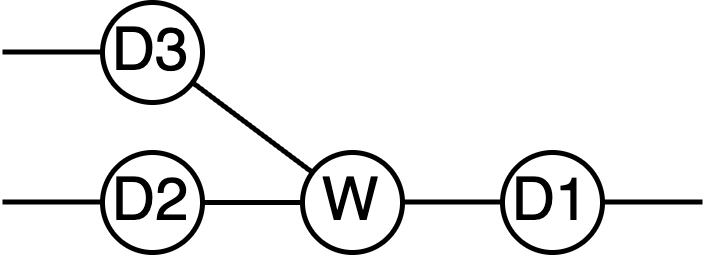
\includegraphics[width=0.7\textwidth]{Assets/Images/4-Entwicklung-der-GFA/Weiche.png}
    \caption{Gleisbild der simulierten Weiche}
    \label{fig:Weiche}
\end{figure}

Alle Achszähler (d1-d3) gehören zu einer Weiche und sind wie in \autoref{fig:Weiche} dargestellt angeordnet. Da die Gleisfreimeldeanlage die Logik einer Fahrstraße nicht überprüft, kann diese Weiche in der Theorie von D1 nach D2, von D1 nach D3 und von D2 nach D3 gestellt werden. \footnote{Die Gegenseiten der Fahrstraßen können natürlich ebenso befahren werden (D2 nach D1, D3 nach D1, D3 nach D2).} Die Tests für die Weichen überprüfen, ob die Gleisfreimeldeanlage korrekt reagiert, wenn eine Weiche gestellt wird. Die Methode \texttt{rail\_vacancy\_assert} wird auch hier verwendet, um die Funktionalität der Gleisfreimeldeanlage zu überprüfen. Der Ausschnitt des Testprogramms ist in \autoref{lst:Testprogramm2} dargestellt.

\begin{lstlisting}[caption={Ausschnitt des Testprogramms für Weichen},label={lst:Testprogramm2},language=C]
  rail_vacancy_assert(v, (rail_contact_point_t *[]){p1, p2, p3, p4}, 4);
  rail_contact_counter_reset(c);

  rail_vacancy_assert(v, (rail_contact_point_t *[]){p4, p3, p2, p1}, 4);
  rail_contact_counter_reset(c);

  rail_vacancy_assert(v, (rail_contact_point_t *[]){p1, p2, p1, p2, p3, p4, p3, p4}, 8);
  rail_contact_counter_reset(c);

  rail_vacancy_assert(v, (rail_contact_point_t *[]){p1, p2, p3, p4, p1, p2, p3, p4}, 8);
  rail_contact_counter_reset(c);

  rail_vacancy_assert_error(v, (rail_contact_point_t *[]){p4, p3, p4, p3, p2, p1, p5, p6}, 8, 4);
  rail_contact_counter_reset(c);

  rail_vacancy_assert_error(v, (rail_contact_point_t *[]){p1, p2, p6, p5, p3, p4, p3, p4}, 8, 3);
  rail_contact_counter_reset(c);

  rail_vacancy_assert(v, (rail_contact_point_t *[]){p1, p2, p5, p6}, 4);
  rail_contact_counter_reset(c);

  rail_vacancy_assert_error(v, (rail_contact_point_t *[]){p1, p2, p2, p1}, 4, 6);
  rail_contact_counter_reset(c);

  rail_vacancy_assert_error(v, (rail_contact_point_t *[]){p2, p1}, 2, 5);
  rail_contact_counter_reset(c);
\end{lstlisting}

Das Programm testet die folgenden Fälle:\footnote{Die Fälle, die mit einem * markiert sind, erwarten einen Fehler}
\begin{itemize}
    \item Ein Zug fährt gerade über die Weiche (D1 nach D2)
    \item Ein Zug fährt in die andere Richtung über die Weiche (D2 nach D1)
    \item Ein Zug mit mehreren Achsen fährt gerade über die Weiche (D1 nach D2)
    \item Zwei Achsen durchfahren die Weiche nacheinander
    \item Zwei Achsen verlassen die Weiche an unterschiedlichen Stellen (D1 nach D2 \& D3)*
    \item Zwei Achsen befahren die Weiche an unterschiedlichen Stellen (D3 \& D2 nach D1)*
    \item Ein Zug fährt im abzweigenden Ast der Weiche (D1 nach D3)
    \item Ein Zug wendet unangekündigt in der Weiche (D1 nach D1)*
    \item Ein Zug verlässt die Weiche ohne in diese eingefahren zu sein (Ausfahrt D1)*
\end{itemize}

Auch hier wird nach jedem Test der Zählerstand des Streckenabschnitts zurückgesetzt, um den nächsten Test vorzubereiten. Die Methode\newline\texttt{rail\_contact\_counter\_reset} wurde bereits in \autoref{text:Entwicklung-der-GFA:Implementierung-der-Gleisfreimeldeanlage:Achszähler:Logik-und-Methoden-der-Achszähler} \nameref{text:Entwicklung-der-GFA:Implementierung-der-Gleisfreimeldeanlage:Achszähler:Logik-und-Methoden-der-Achszähler} vorgestellt.